\section{Results}
\label{sec:results}

\begin{table}[t!]
	\centering
	\begin{tabular}{|c|ccc|}
		\hline
		Classification & CLP & CENS & CRP \\
		\hline
		Template (binary) & 24.17\% & 20.08\% & 24.96\% \\
		Template (harmonic) & 23.04\% & 17.79\% & 20.38\% \\
		GMM & 14.58\% & 6.94\% & 11.81\% \\
		\hline
		SVM (linear) & 13.61\% & 6.39\% & 12.64\% \\
		SVM (poly) & 10.56\% & 4.17\% & 7.92\% \\
		SVM (RBF) & 10.00\% & 4.31\% & 7.78\% \\
		\hline
	\end{tabular}
	\caption{Error results of the first part of the tests (single chord recognition)}
	\label{tab:singleChordResults}
	\vspace{-6mm}
\end{table}
%
For the first part of the experiment we simply run all the different classification methods explained in Section~\ref{sec:setup} randomly splitting the dataset into $70\%$ training and $30\%$ testing. The results can be clearly seen in Tab.~\ref{tab:singleChordResults}. Note that the first approach (templates) yields very poor results even in such an idealized scenario, while the more advanced \textit{Harmonic Templates} improved a little bit performance over the simple \textit{Binary} ones. The jump to the more advanced GMMs is pretty clear as much as the one to SVMs. Overall, CENS features have by far the best error rates.
%
\begin{table}[b]
	\centering
	\subfigure[Before the processing with HMM]{
		\centering
		\begin{tabular}{|c |c c c|}
			\hline
			$r_{test}$ & CENS & CLP & CRP\\ \hline
			0.1 & 49.46\% & 47.39\% & 62.06\%\\
			0.2 & 46.57\% & 60.00\% & 63.76\%\\
			0.3 & 47.65\% & 56.91\% & 58.03\%\\
			\hline
		\end{tabular}
		\label{tab:resultbeforeHMM}
	}\\
	\subfigure[After the processing with HMM]{
		\centering
		\begin{tabular}{|c |c c c|}
			\hline
			$r_{test}$ & CENS & CLP & CRP\\ \hline
			0.1 & 44.39\% & 45.02\% & 56.41\%\\
			0.2 & 42.96\% & 59.19\% & 59.67\%\\
			0.3 & 41.79\% & 54.84\% & 52.04\%\\
			\hline
		\end{tabular}
		\label{tab:resultafterHMM}
	}
	\vspace{-3mm}
	\caption{Error results of the first part of the tests (full song chord recognition)}
	\label{tabs:results_2}
	\vspace{-6mm}
\end{table}
%
For the second part of the experiment we got two different kind of outputs for each song, which are $\mathcal{L}_{SVM}$ and $\mathcal{L}_{HMM}$. In order to verify the quality of our results we compared them with  $\mathcal{L}_{Harte}$. Given $\mathcal{L}_{SVM}$ ($\mathcal{L}_{HMM}$) and $\mathcal{L}_{Harte}$ for a certain value of $r_{test}$ and for a certain extracted feature we computed the error probability as a simple normalized \textit{Hamming distance}.

In Tabs.~\ref{tabs:results_2} we can see the results before and after the HMM processing. In both cases we show different outputs depending on the testing rate $r_{test}$ and on the chosen extracted feature.
%
\begin{figure}[t]
	\centering
	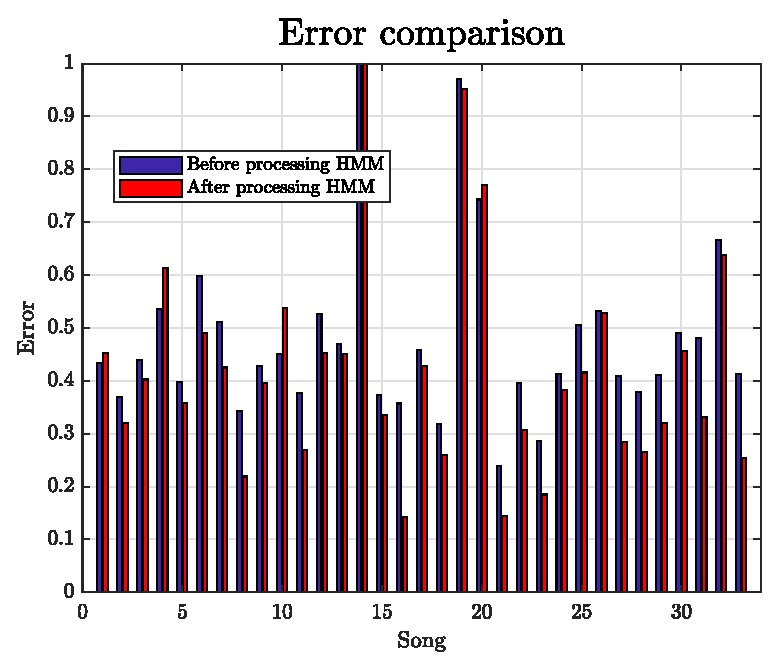
\includegraphics[width=0.4\textwidth]{img/Result_HMM/CENS/plot03071}
	\vspace{-3mm}
	\caption{Error comparison using CENS features and $r_{test}=0.3$}
	\label{fig:compareerror}
	\vspace{-6mm}
\end{figure}
\begin{figure}[tb]
	\centering
	\subfigure[Chords variation per song using CENS features and $r_{test}=0.1$]{
		\centering
		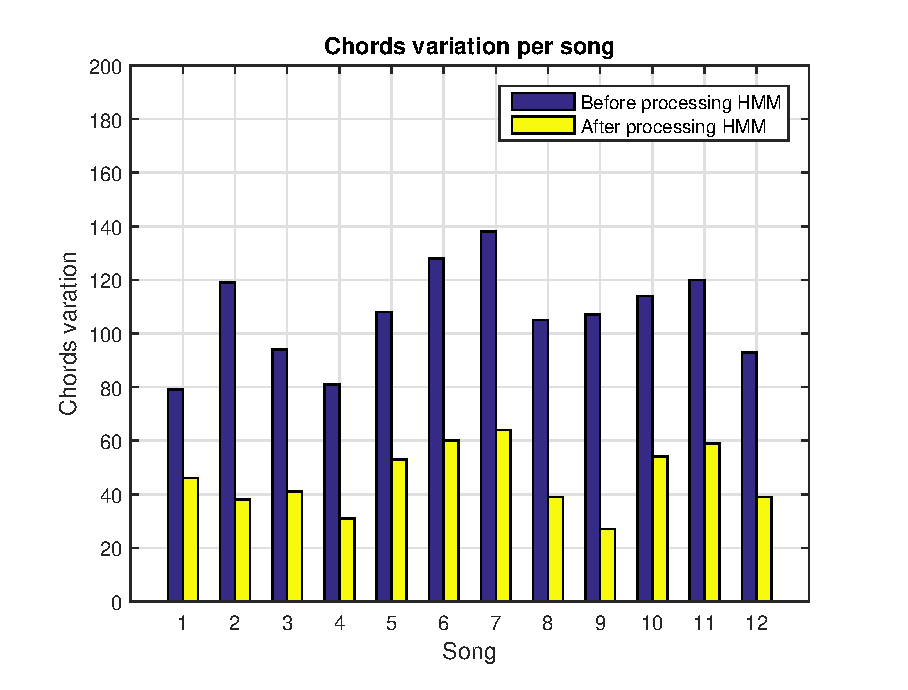
\includegraphics[width=0.4\textwidth]{img/Result_HMM/SMOOTHING/SmoothPerSongCENS0109}
		\label{fig:smoothmulti}
	}
	\\
	\subfigure[Chord variation in a single song using CENS features and $r_{test}=0.1$]{
		\centering
		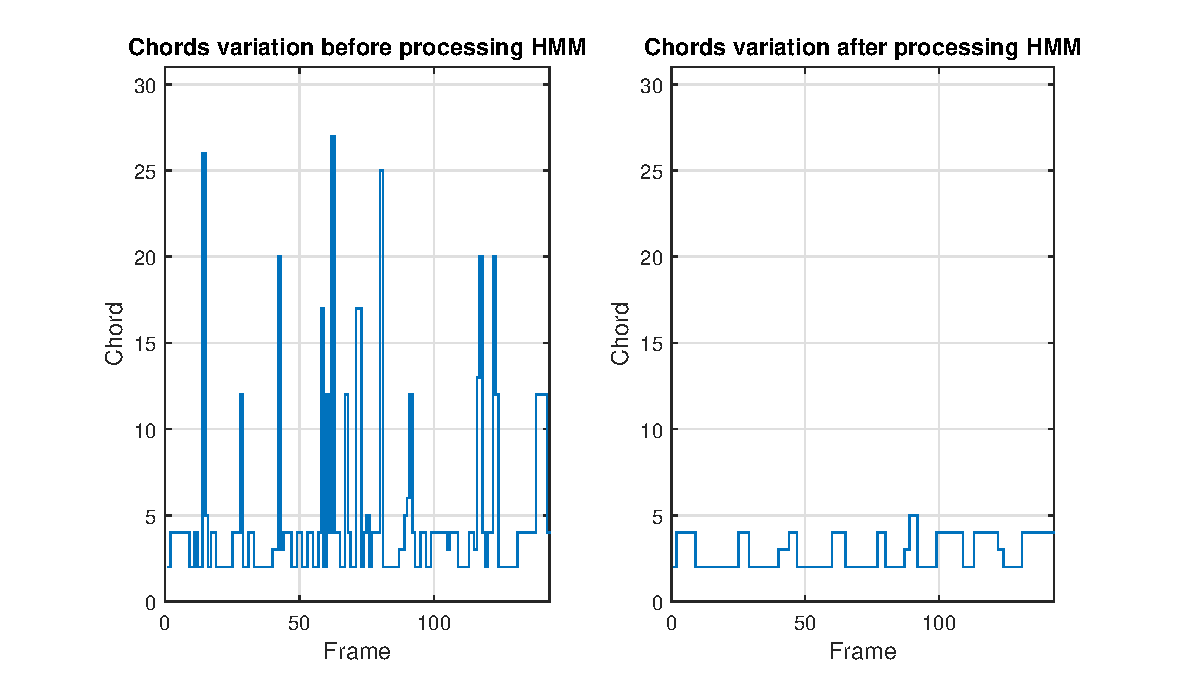
\includegraphics[width=0.4\textwidth]{img/Result_HMM/SMOOTHING/SmoothSingleSongCENS0109}
		\label{fig:smoothsingle}
	}
	\vspace{-3mm}
	\caption{Results of the smoothing using HMMs}
	\vspace{-6mm}
\end{figure}
%
From these results we make the following observations. First, CENS features performed the best. Second, HMM proved to be able to enhance the results with respect to MC-SVM alone in all the cases. This is not obvious since we worked with features of multi-instrumental sounds including also vocal and drum parts. Indeed the chords prediction of some songs often isn't improved but is aggravated. We show this by comparing the two different results obtained with the same $\mathcal{D}_{train}$ as done in Fig.~\ref{fig:compareerror}.
%
We concluded that HMM don't always improve our result for every single song. It is able to do so only in average. However what HMM is able to do for each song is reduce the chords variation. We define chord variation as the number of times that a chord sequence varies within the same song. This value decreases, since HMM tends to correct the most improbable outputs generated by MC-SVM. We find confirmation to this assumption looking at Figs.~\ref{fig:smoothmulti},\ref{fig:smoothsingle}. In particular in Fig.~\ref{fig:smoothsingle} we can see how HMM removes the impulsive chord variations which tend to be quite unlikely.
